
\hwpart{II}{Implement DDPM (25 points)}
Now it's time to build your first diffusion model! Take a good look at the starter code and start building! Remember, you are free to add, delete and modify any and all parts of the starter code to fit your preference.

\question{Building Intuition}{optional, 0}

Before diving into the full scale training, it is generally a good idea to build some intuitions of the algorithm with some toy examples as they are easier to debug.

\subq{a}{0} We have prepared a Jupyter notebook \textit{01\_1d\_playground.ipynb} for you to experiment with 1D toy data. This notebook contains some options of mixture of Gaussians and their visualizations, you can try out your algorithm first in this playground.

\subq{b}{0} Full scale training can be difficult to debug sometimes, and that's why in \textit{train.py} we also provide an argument flag, \textit{-\--overfit-single-batch}, for you to toggle an experiment where you overfit to a single batch of data for sanity checking. You should be able to iterate your model a lot faster with this experiment than full scale training.

\question{Implementation}{25}

Now implement DDPM for real! The starter code provides the skeleton, and your job is to fill in the core algorithm.
Remember: this is your codebase. Feel free to modify any part of the starter code to fit your preferences. Add helper functions, reorganize files, change the config structure... whatever helps. The only requirement is that your final code runs and produces good results.

The starter code provides a detailed guideline on which files are provided and which files are the ones that need your implementation. Go check it out!

\subq{a}{5} Train your DDPM model to convergence. You may use either the provided configs or your own. Report:
\begin{enumerate}
    \item Model size
    \item Batch size
    \item Total training iterations
    \item Training loss curve
    \item Compute cost (GPU hours)
\end{enumerate}
\answerbox{}{
I trained the DDPM on the provided CelebA 64x64 subset
(\texttt{electronickale/cmu-10799-celeba64-subset}) using the Colab config in
\texttt{configs/ddpm\_colab.yaml}. The model is a timestep-conditioned U-Net
with \textbf{15,605,635} parameters (\(\approx 15.61\)M).

\begin{center}
\begin{tabular}{ll}
\toprule
Batch size & 64 \\
Training iterations & 100,000 \\
Image shape & \(3 \times 64 \times 64\) \\
DDPM timesteps & 1000 \\
Beta schedule & linear, \(10^{-4}\) to \(2 \times 10^{-2}\) \\
Optimizer & AdamW, learning rate \(2 \times 10^{-4}\) \\
EMA decay & 0.9999 \\
Mixed precision & enabled \\
Final checkpoint & \texttt{ddpm\_final.pt} \\
\bottomrule
\end{tabular}
\end{center}

Training was interrupted by Colab runtime disconnects and resumed from saved
checkpoints. The checkpoints restore model, optimizer, EMA, AMP scaler, step,
and config state. The run used approximately \textbf{2.6 GPU-hours} for the
actual training loop, based on the checkpoint timestamps and tqdm wall-clock
output: roughly 1.5 GPU-hours for steps 0--60k and roughly 1.1 GPU-hours for
steps 60k--100k. This estimate excludes package installation, dataset download,
manual reconnect time, and post-training evaluation.

\begin{center}
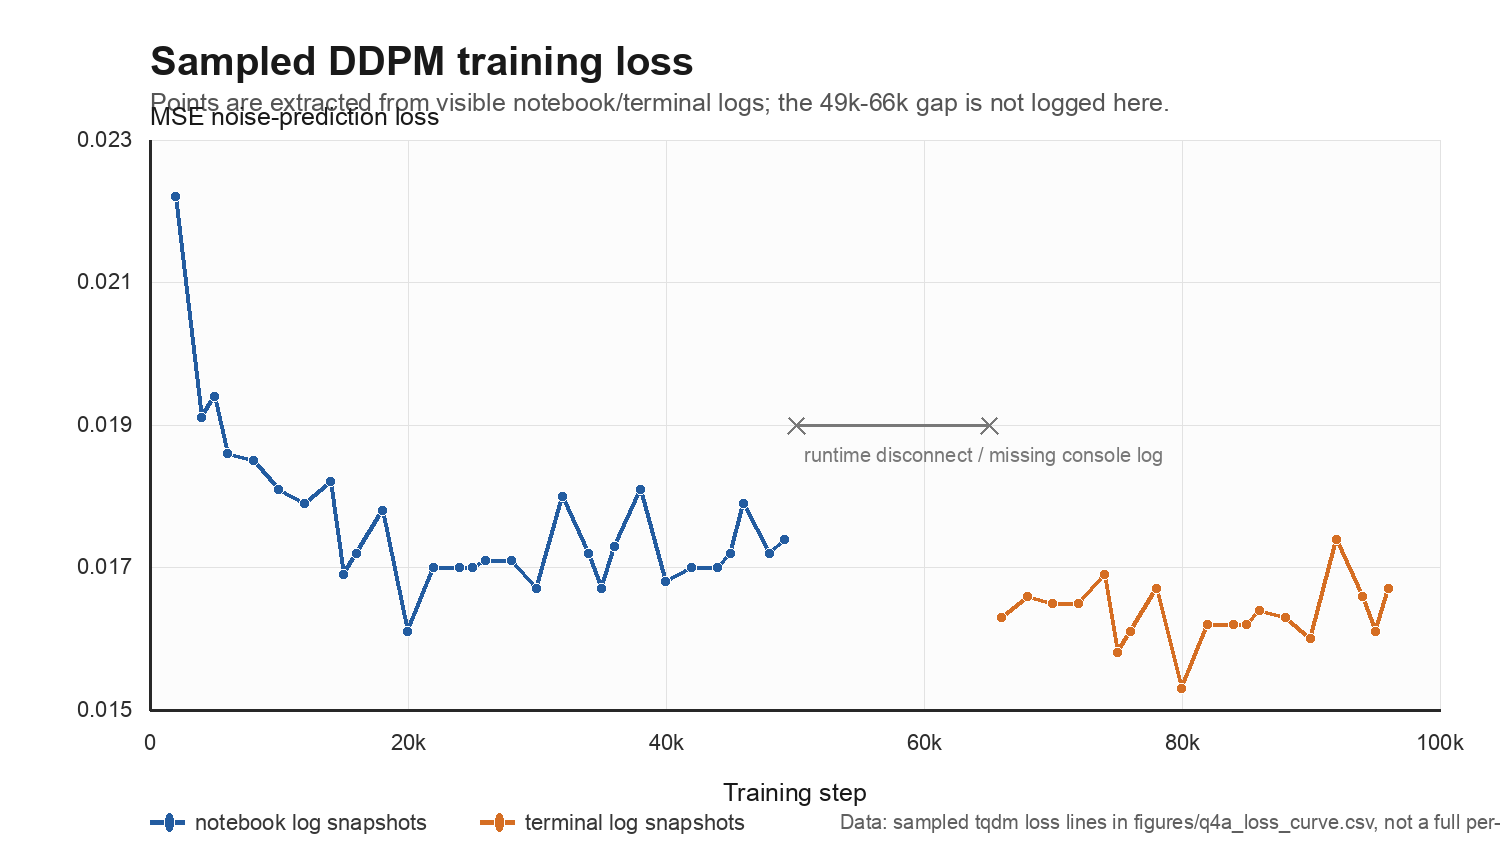
\includegraphics[width=0.78\linewidth]{figures/q4a_loss_curve.png}
\end{center}

The plotted trace is a sampled training-loss trace rather than a full per-step
metric log. The points come from the visible tqdm lines in the Colab notebook
and terminal output, and the gap between the first and resumed sessions is left
explicitly unconnected in the figure. The denoising MSE drops quickly in the
first few thousand steps and then stays mostly around \(1.6 \times 10^{-2}\) to
\(1.8 \times 10^{-2}\). The extracted points are saved in
\texttt{figures/q4a\_loss\_curve.csv}.
}
\includeanswer{q4a}

\subq{b}{10} Generate a grid of 16 samples from your trained model. Include this grid below.
\answerbox{}{
The following grid was generated from the final EMA checkpoint after 100,000
training iterations.

\begin{center}
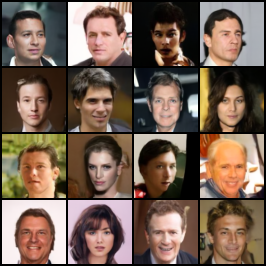
\includegraphics[width=0.72\linewidth]{figures/q4b_samples_0100000.png}
\end{center}
}
\includeanswer{q4b}

\subq{c}{10} Evaluate your model KID with 1k samples and report your KID score (both mean and std). You should be able to obtain KID < 0.005 with single L40S GPU training for a few hours.
\answerbox{}{
\textbf{Pending.} The final checkpoint and 16-sample grid have been exported
locally, but the 1k-sample KID evaluation still needs to be run on Colab because
standard DDPM sampling requires 1000 reverse U-Net evaluations per generated
batch. The updated \texttt{part\_ii.ipynb} contains a Colab KID section that:
generates 1000 EMA samples from \texttt{ddpm\_final.pt}, exports 1000 real
CelebA subset images, and evaluates KID with \texttt{torch-fidelity}. The result
to report here is the \texttt{kernel\_inception\_distance\_mean} and
\texttt{kernel\_inception\_distance\_std} printed by that cell.
}
\includeanswer{q4c}

\subq{d}{0} Provide a zip file of your code through Gradescope ``Homework 1 Code'' assignment. Make sure your code is runnable because we may run it to verify your results, and do not include any large files such as model checkpoints or dataset files. If you do not provide a zip file for your code, you will receive 0 point on Part II and Part IV of this homework.
\answerbox{}{
The code zip should include the runnable repository code and configs, but should
\textbf{exclude} generated datasets, logs, samples, and large checkpoints such as
\texttt{ddpm\_final.pt}. I keep the trained model and generated figures outside
the code zip and submit them only through the written report or separate
artifact workflow if requested.
}
\includeanswer{q4d}
